\hypertarget{introduction}{%
\section{Introduction}\label{introduction}}

Ecological networks are a useful way to think about ecological systems
in which species or organism interact (Delmas et al. 2018; Poisot,
Stouffer, and Kéfi 2016), and recently there has been an explosion of
interest in their dynamics across large temporal scales (Baiser et al.
2019; Tylianakis and Morris 2017), especially alongside environmental
gradients (Pellissier et al. 2017; Trøjelsgaard and Olesen 2016).

Thompson and Gonzalez (2017) need movement + future climate for
predictions, can't do with data scarcity

This interest has motivated two efforts: an expansion of the tools used
to investigate ecological networks, and an increase data collection
efforts. In order for both of these efforts to progress, we need a means
for ecologists to share and access high-quality network data. Mangal
responds to this need, by providing an online database of open network
data. Our purpose in the current document is threefold:

\begin{enumerate}
\def\labelenumi{\arabic{enumi}.}
\tightlist
\item
  to describe updates and improvements to the Mangal project
\item
  to demonstrate the kinds of analyses possible through worked examples
\item
  to highlight the need for more empirical network data, especially in
  undersampled regions.
\end{enumerate}

\hypertarget{synthesis-on-ecological-networks-is-rising}{%
\subsection{Synthesis on ecological networks is
rising}\label{synthesis-on-ecological-networks-is-rising}}

Borrett, Moody, and Edelmann (2014)

Synthesizing ecological data presents important challenges and also some
exciting opportunities. Mangal is well suited to offer such
opportunities in the study of ecological networks.

\begin{itemize}
\tightlist
\item
  A major challenge to ecological synthesis is generalizing from samples
  to the behaviour of ecological systems
\item
  two obstacles to such generalizing in ecological systems: data
  coverage and data quality

  \begin{itemize}
  \tightlist
  \item
    data coverage: are data collected from every relevant system?
  \item
    data quality: are data fit-for-purpose? Two particular aspects of
    quality

    \begin{itemize}
    \tightlist
    \item
      taxonomic resolution
    \item
      sampling effort
    \end{itemize}
  \end{itemize}
\end{itemize}

\hypertarget{the-need-for-an-integrated-networks-database}{%
\subsection{The need for an integrated networks
database}\label{the-need-for-an-integrated-networks-database}}

Mangal is an actively developed project which has recently been expanded
and improved. Poisot et al. (2016) -- original mangal paper

\begin{itemize}
\tightlist
\item
  An earlier manuscript (Poisot et al 2015 {[}tk{]}) described Mangal as
  an online platform allowing ecologists to share data about ecological
  networks
\item
  New technical improvements include:
\item
  New data
\item
  number and amount of new information
\item
  web API for better data access, and two packages (one in Julia, the
  other in R) for accessing these data.
\item
  Mangal in its current form offers open network data that is ready to
  support synthesis at many scales.
\end{itemize}

\begin{itemize}
\item
  \emph{Coverage in geographic space.} Mangal now contains information
  from all over the world, and from every continent except Antarctica. 
\item
  \emph{Coverage in climate space} Early ecologists identified the
  earth's biomes based on combinations of temperature and precipitation.
  Here we demonstrate that Mangal datasets have been sampled from across
  these different biomes. In doing so, we also demonstrate how climate
  data can be downloaded and combined with Mangal records. 
\end{itemize}

This database documents the impressive efforts of (generations of?)
ecologists who have sampled nearly every continent and climatic zone, as
well as various taxonomic groups and interaction types.

\hypertarget{global-trends-in-ecological-networks-description}{%
\section{Global trends in ecological networks
description}\label{global-trends-in-ecological-networks-description}}

\hypertarget{network-coverage-is-accelerating}{%
\subsection{Network coverage is
accelerating}\label{network-coverage-is-accelerating}}

\begin{figure}
\centering
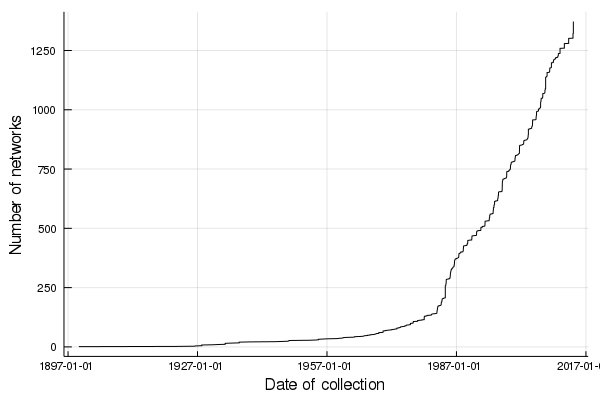
\includegraphics{figures/figure_01_a.png}
\caption{fig1\label{fig:temporal}}
\end{figure}

\hypertarget{networks-follow-the-same-scaling}{%
\subsection{Networks follow the same
scaling}\label{networks-follow-the-same-scaling}}

Brose et al. (2004)

\begin{figure}
\centering
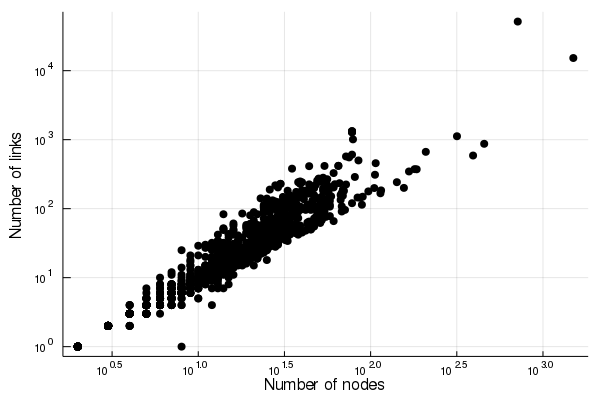
\includegraphics{figures/figure_01_b.png}
\caption{fig1 ref\label{fig:lssl}}
\end{figure}

\hypertarget{different-types-of-networks-have-been-studied-in-different-biomes}{%
\subsection{Different types of networks have been studied in different
biomes}\label{different-types-of-networks-have-been-studied-in-different-biomes}}

Whittaker (1962)

\begin{figure}
\centering
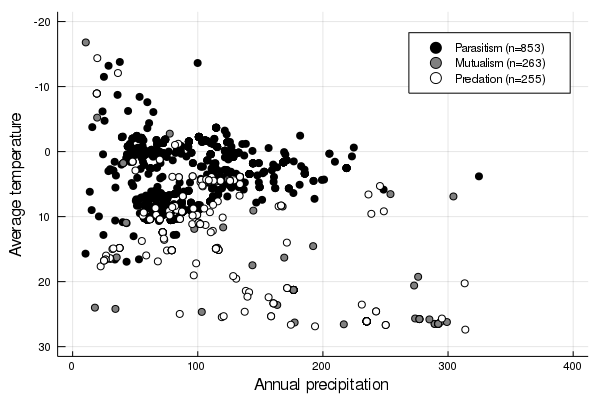
\includegraphics{figures/figure_02.png}
\caption{List of networks across biomes\label{fig:biomes}}
\end{figure}

\hypertarget{eccentricity-of-climate}{%
\subsection{Eccentricity of climate}\label{eccentricity-of-climate}}

\begin{figure}
\centering
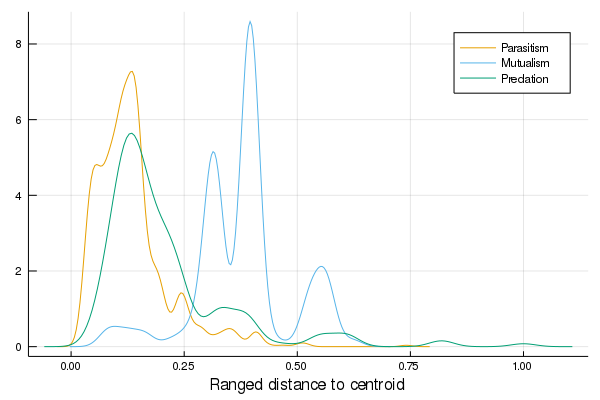
\includegraphics{figures/figure_05_b.png}
\caption{tk\label{fig:ecc}}
\end{figure}

\hypertarget{need-to-find-a-title}{%
\subsection{NEED TO FIND A TITLE}\label{need-to-find-a-title}}

Distance issues

\begin{figure}
\centering
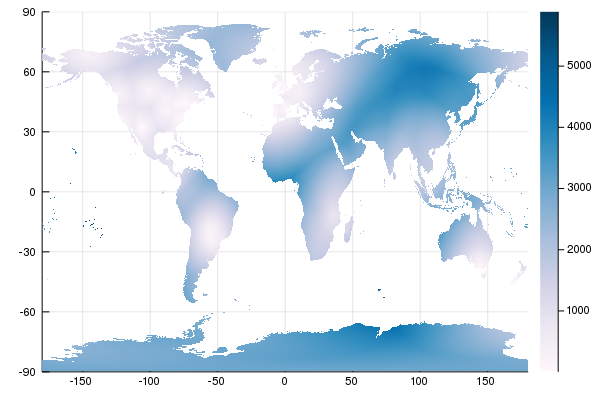
\includegraphics{figures/figure_03_a.png}
\caption{tk\label{fig:distance}}
\end{figure}

Climate analogue

\begin{figure}
\centering
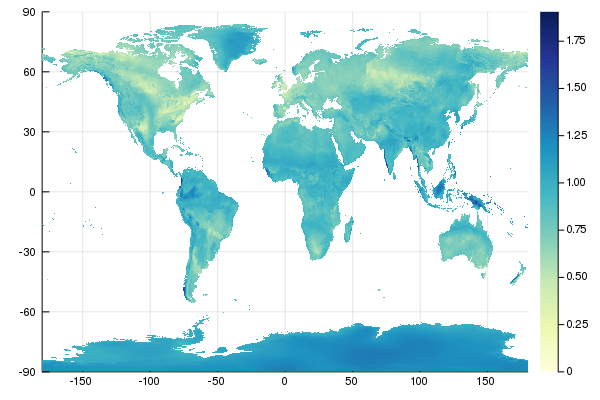
\includegraphics{figures/figure_03_b.png}
\caption{tk\label{fig:analog}}
\end{figure}

\hypertarget{conclusions}{%
\section{Conclusions}\label{conclusions}}

\hypertarget{reducing-uncertainty-through-analogues}{%
\subsection{reducing uncertainty through
`analogues'}\label{reducing-uncertainty-through-analogues}}

When we lack direct observation of a community, often we must resort to
the use of `analog' communities -- that is, communities which are
similar in space or environment which have been sampled.

\begin{itemize}
\tightlist
\item
  Communities may be similar in at least two ways -- close in space, or
  close in climate
\item
  similarity may result in some (?) similarity in network structure,
  even if species different.
\item
  Always some uncertainty in such comparisons
\item
  reflects the need for more data gathering, can be used to target
  efforts
\end{itemize}

\hypertarget{future-of-network-ecology}{%
\subsection{Future of network ecology}\label{future-of-network-ecology}}

Use this spatial gaps for sampling recommendations

\hypertarget{more-complete-analyses}{%
\subsection{more complete analyses}\label{more-complete-analyses}}

We have only shown some high-level summaries of the data here; many
possibilities remain.

\hypertarget{more-data-collection}{%
\subsection{more data collection}\label{more-data-collection}}

We have demonstrated the considerable coverage of Mangal; however, our
summary also highlights important data-collection needs. In particular,
we need better information about (mutualists, desert food webs?)

\hypertarget{active-development-and-data-contribution}{%
\subsection{Active development and data
contribution}\label{active-development-and-data-contribution}}

This is an open-source project: all data and all code supporting this
are available on the Mangal project GitHub organization. Our hope is
that the success of this project will encourage similar efforts within
other parts of the ecological community. In addition, we hope that this
project will encourage the recognition of the contribution that software
creators make to ecological research.

\hypertarget{data-quality-sampling-effort-and-taxonomy}{%
\subsection{Data quality: sampling effort and
taxonomy}\label{data-quality-sampling-effort-and-taxonomy}}

Sampling effort and taxonomic detail are two very challenging but
important part of any ecological dataset. The datasets in Mangal
represent some of the most detailed studies of ecological networks
available. * measures of network structure may be particularly sensitive
to the amount of sampling effort * repeat sampling may be necessary to
capture a ``saturation'' of interactions. * we present some
visualization of the sampling coverage of Mangal {[}tk{]} * High
taxonomic resolution is difficult to achieve in ecology, especially
depending on the sampling method used (e.g.~gut contents vs
observations). We present a breakdown of the taxonomic resolution of
Mangal. * Ecological networks occur in various kinds, but they are not
all equally well sampled. We present a breakdown of the number of
parasitic, mutualistic and predator-prey networks sampled in Mangal

\hypertarget{references}{%
\section*{References}\label{references}}
\addcontentsline{toc}{section}{References}

\hypertarget{refs}{}
\leavevmode\hypertarget{ref-BaisGrav19}{}%
Baiser, Benjamin, Dominique Gravel, Alyssa R. Cirtwill, Jennifer A.
Dunne, Ashkaan K. Fahimipour, Luis J. Gilarranz, Joshua A. Grochow, et
al. 2019. ``Ecogeographical Rules and the Macroecology of Food Webs.''
\emph{Global Ecology and Biogeography} 0 (0).
\url{https://doi.org/10.1111/geb.12925}.

\leavevmode\hypertarget{ref-BorrMood14}{}%
Borrett, Stuart R., James Moody, and Achim Edelmann. 2014. ``The Rise of
Network Ecology: Maps of the Topic Diversity and Scientific
Collaboration.'' \emph{Ecological Modelling} 293 (December): 111--27.
\url{https://doi.org/10.1016/j.ecolmodel.2014.02.019}.

\leavevmode\hypertarget{ref-BrosOstl04}{}%
Brose, Ulrich, Annette Ostling, Kateri Harrison, and Neo D. Martinez.
2004. ``Unified Spatial Scaling of Species and Their Trophic
Interactions.'' \emph{Nature} 428 (6979): 167--71.
\url{https://doi.org/10.1038/nature02297}.

\leavevmode\hypertarget{ref-DelmBess18}{}%
Delmas, Eva, Mathilde Besson, Marie-Hélène Brice, Laura A. Burkle,
Giulio V. Dalla Riva, Marie-Josée Fortin, Dominique Gravel, et al. 2018.
``Analysing Ecological Networks of Species Interactions.''
\emph{Biological Reviews}, June, 112540.
\url{https://doi.org/10.1111/brv.12433}.

\leavevmode\hypertarget{ref-PellAlbo17}{}%
Pellissier, Loïc, Camille Albouy, Jordi Bascompte, Nina Farwig,
Catherine Graham, Michel Loreau, Maria Alejandra Maglianesi, et al.
2017. ``Comparing Species Interaction Networks Along Environmental
Gradients.'' \emph{Biological Reviews of the Cambridge Philosophical
Society}, September. \url{https://doi.org/10.1111/brv.12366}.

\leavevmode\hypertarget{ref-PoisBais16}{}%
Poisot, Timothée, Benjamin Baiser, Jennifer A. Dunne, Sonia Kéfi,
François Massol, Nicolas Mouquet, Tamara N. Romanuk, Daniel B. Stouffer,
Spencer A. Wood, and Dominique Gravel. 2016. ``Mangal - Making
Ecological Network Analysis Simple.'' \emph{Ecography} 39 (4): 384--90.
\url{https://doi.org/10.1111/ecog.00976}.

\leavevmode\hypertarget{ref-PoisStou16}{}%
Poisot, Timothée, Daniel B. Stouffer, and Sonia Kéfi. 2016. ``Describe,
Understand and Predict: Why Do We Need Networks in Ecology?''
\emph{Functional Ecology} 30 (12): 1878--82.
\url{https://doi.org/10.1111/1365-2435.12799}.

\leavevmode\hypertarget{ref-ThomGonz17}{}%
Thompson, Patrick L., and Andrew Gonzalez. 2017. ``Dispersal Governs the
Reorganization of Ecological Networks Under Environmental Change.''
\emph{Nature Ecology \& Evolution} 1 (May): 0162.
\url{https://doi.org/10.1038/s41559-017-0162}.

\leavevmode\hypertarget{ref-TrojOles16}{}%
Trøjelsgaard, Kristian, and Jens M. Olesen. 2016. ``Ecological Networks
in Motion: Micro- and Macroscopic Variability Across Scales.''
\emph{Functional Ecology} 30 (12): 1926--35.
\url{https://doi.org/10.1111/1365-2435.12710}.

\leavevmode\hypertarget{ref-TyliMorr17}{}%
Tylianakis, Jason M., and Rebecca J. Morris. 2017. ``Ecological Networks
Across Environmental Gradients.'' \emph{Annual Review of Ecology,
Evolution, and Systematics} 48 (1): 25--48.
\url{https://doi.org/10.1146/annurev-ecolsys-110316-022821}.

\leavevmode\hypertarget{ref-Whit62}{}%
Whittaker, Robert H. 1962. ``Classification of Natural Communities.''
\emph{Botanical Review} 28 (1): 1--239.
\url{https://www.jstor.org/stable/4353649}.
